\documentclass[conference]{IEEEtran}
% \IEEEoverridecommandlockouts
% The preceding line is only needed to identify funding in the first footnote. If that is unneeded, please comment it out.
\usepackage{cite}
\usepackage{amsmath,amssymb,amsfonts}
\usepackage{algorithmic}
\usepackage{graphicx, float}
\usepackage{textcomp}
\usepackage{xcolor}
\usepackage{url}
\def\BibTeX{{\rm B\kern-.05em{\sc i\kern-.025em b}\kern-.08em
    T\kern-.1667em\lower.7ex\hbox{E}\kern-.125emX}}
\begin{document}

\title{Conference Paper Title*\\
{\footnotesize \textsuperscript{*}Note: Sub-titles are not captured in Xplore and
should not be used}
\thanks{Identify applicable funding agency here. If none, delete this.}
}

\author{\IEEEauthorblockN{1\textsuperscript{st} Alex Booth}
\IEEEauthorblockA{\textit{School of Computing, Science and Engineering} \\
\textit{The University of Salford}\\
City, Country \\
email address or ORCID}}

\maketitle

\begin{abstract}
This document is a model and instructions for \LaTeX.
This and the IEEEtran.cls file define the components of your paper [title, text, heads, etc.]. *CRITICAL: Do Not Use Symbols, Special Characters, Footnotes, 
or Math in Paper Title or Abstract.
\end{abstract}cccc

\section{Introduction}
    This document is a model and instructions for \LaTeX.
    Please observe the conference page limits. 

\section{Theory}
    \subsection{Impulse Responses}
        To compensate for the frequency response of a room so that a listener in the room hears the output of a loudspeaker without any coloration of the sound by the room, one must first find and quantify the way the room effects sound produced by the speaker.
        When approaching this task using digital signal processing, finding the room's impulse response allows us to quantify the way it affects any input impulse.
        A digital impulse is a single sample signal with a sample value of 1.
        A more precise mathematical definition is given in Eq.\ref{uSample}:
        \begin{equation}\label{uSample}
            \delta[n] = 
            \begin{cases}
                0, n \neq 0\\
                1, n = 0
            \end{cases}
        \end{equation}
        By knowing the response of a system when the input is an impulse $\delta[n]$, allows the response of the system to any input to be predicted, so long as the system is both linear and shift-invariant \cite{OPPENHEIM}.
        This response to $\delta[n]$ is known as the impulse response, $h[n]$.
        In this digital model, the room's frequency response is effectively a series of filters and so it will be both linear and shift-invariant.
        By convolving $h[n]$ with any input $x[n]$, the output $y[n]$ of the signal flow can be found. 
        The convolution in the digital domain is formulated as a sum, as opposed to the continuous time domain where it is an integral.
        The digital convolution sum is shown in Eq.\ref{conv}
        \begin{equation}\label{conv}
            y[n] = \sum_{k=-\infty}^\infty x[k] h[n-k]
        \end{equation}
        So by computing the convolution sum of an input signal with the impulse response of the room, the output of the room can be found, and thus the effect of the room on the frequency response of a signal.
    \subsection{Test Signals}
        To test the effectiveness of a compensation filter, test signals to be used as input must be devised.
        The frequency and amplitude components of test signals are important, such that the effectiveness of the filter is tested over as wide a range of frequencies and amplitudes as possible.
        Two common input signals used to test digital filters are 'chirps' and 'bursts'.
        A chirp is a pure sine wave signal swept from low to high frequency over it's signal length; it can be swept linearly or logarithmically, and can cover any frequency range as required.
        A linearly swept sine is defined by Eq.\ref{chirp}, where $\phi_0$ is initial phase, $t$ is time, and $f_0$ is initial frequency.
        \begin{equation}\label{chirp}
            x[t] = \sin{[\phi_0 + 2\pi(\frac{c}{2} t^2 + f_0 t)]}
        \end{equation}
        A burst is a short length of pink noise.
        A digital noise signal is non-deterministic and statistically random in it's current sample value, as so it cannot be described to have a frequency or period, as it is almost impossible for it to repeat over a given time period \cite{OPPENHEIM376}.
        This randomness can instead be quantified with a standard deviation $\sigma$, and probability of frequency \& magnitude components arising throughout the signal.
        White noise is the most basic noise signal, with every frequency sharing an equal probability of arising at all times throughout the signal; it has constant power spectral density \cite{CARTER}
        Pink noise, does not have a constant equal probability for any frequency to arise in the signal.
        \begin{figure}[H]
            \centering
            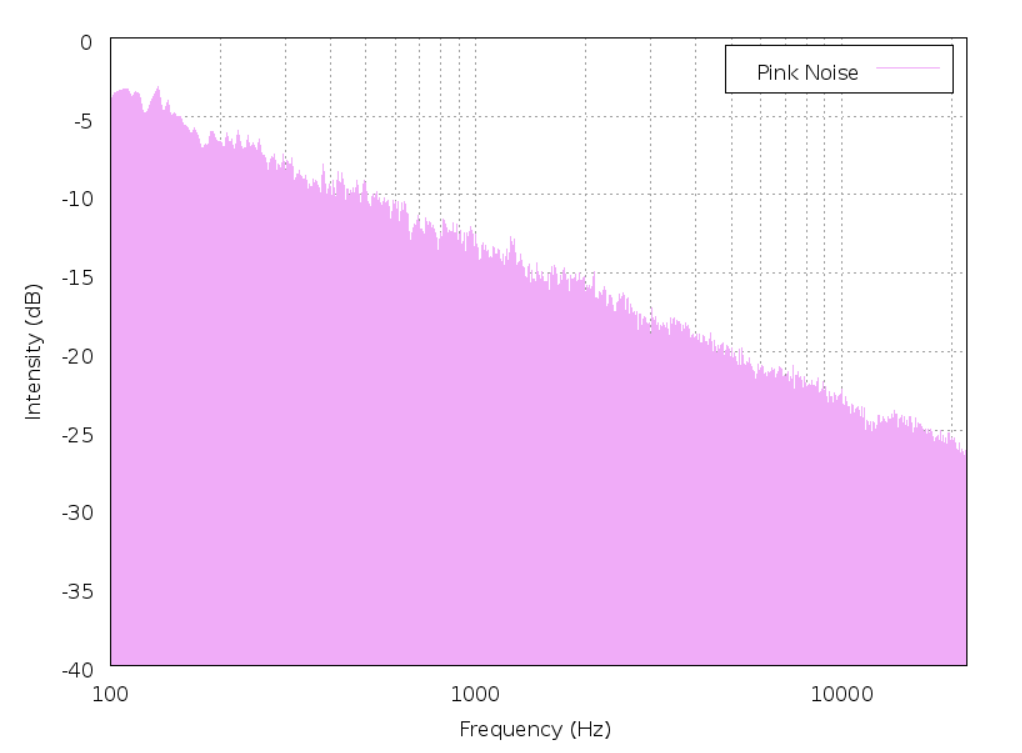
\includegraphics[scale = 0.35]{resources/PinkNoise.png}
            \caption{Frequency Response of Pink Noise \cite{AFIELDS}}
        \end{figure}
        Instead, pink noise's power spectral density is inversely proportional to the frequency of the signal.
        Using pink noise as a test signal is preferred over white noise, as the roll-off in average amplitude over frequency generally follows the equal loudness curve - where the human auditory experience is more sensitive to high frequencies \cite{GENELEC}.
        With white noise the high frequencies naturally dominate the human auditory experience; the frequency roll-off of pink noise compensates for this.
        
    \subsection{Digital Filters}
        In the continuous time audio domain, filters are applied using either passive or active circuits.
        Loudspeakers often use these analog electronic filters to cross-over the optimal frequency pass-bands of a pair of drivers to create an optimum combined system response.
        In the digital, discrete-time domain, filters are realized as linear, shift-invariant systems.
        Digital filters fall into two categories, finite impulse response (FIR) and infinite impulse response (IIR).
        As their names imply, the main difference between the two digital filter types is their impulse responses.
        An IIR filter's  signal flow is recursive and thus - when fed an impulse of $\delta[n]$, the impulse response $h[n]$ is infinitely long.
        An FIR filter has a feed-forward signal flow and so is not recursive and has a finitely long impulse response.
        Equation \ref{FIR} shows the general form of an FIR filter, where the output is equal the the input $x[n]$ convolved with the impulse response of the filter $h[n]$ \cite{JORDAN}:
        \begin{equation}\label{FIR}
            y[n] = \sum_{k=0}^N h_k x_{n-k}
        \end{equation}
        % Figure \ref{BLOCK} shows a block diagra
        yoooooo
        
\section{Methodology}

\section{Results}

\bibliographystyle{plain}
\bibliography{theBib}

\end{document}
